\documentclass[UTF8]{ctexart}

\usepackage{titlesec}
\usepackage{geometry}
\geometry{a4paper,left=3cm,right=3cm,bottom=1cm,top=1cm}
\usepackage{graphicx}
\usepackage{epstopdf}
\usepackage{indentfirst}
\usepackage{caption}
\usepackage{amsmath} %数学公式
\usepackage{amsthm}
\usepackage{graphics}

\usepackage{bmpsize}

\begin{document}
	\section{实验原理和目的}
	
	
	
	\section{实验结果}

	\begin{figure}
		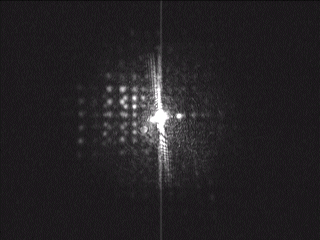
\includegraphics{1.jpg}
	\end{figure}
	
	\begin{figure}[h]
		\centering
		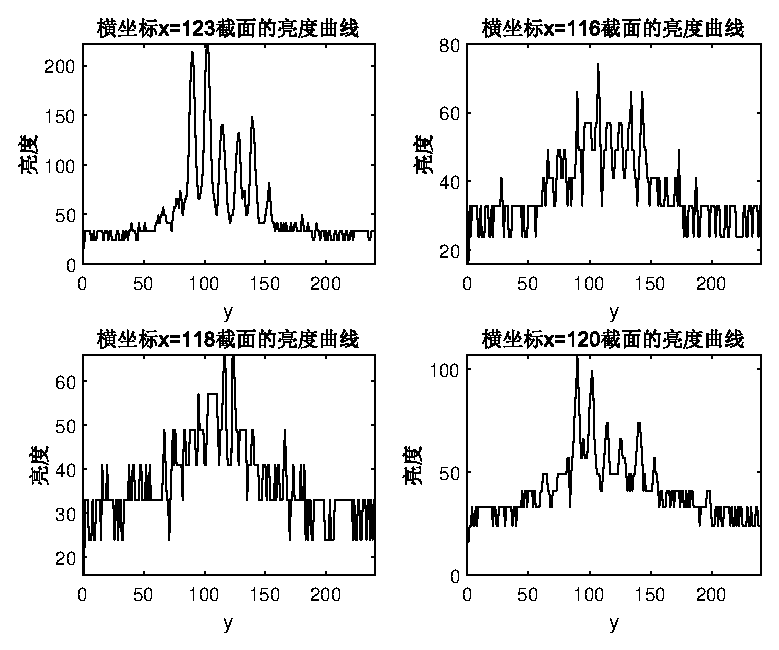
\includegraphics{beforeDOE.eps}
		\caption{未加DOE的亮度曲线}\label{未加DOE亮度}
	\end{figure}
	
	\begin{figure} [h]
		\centering
		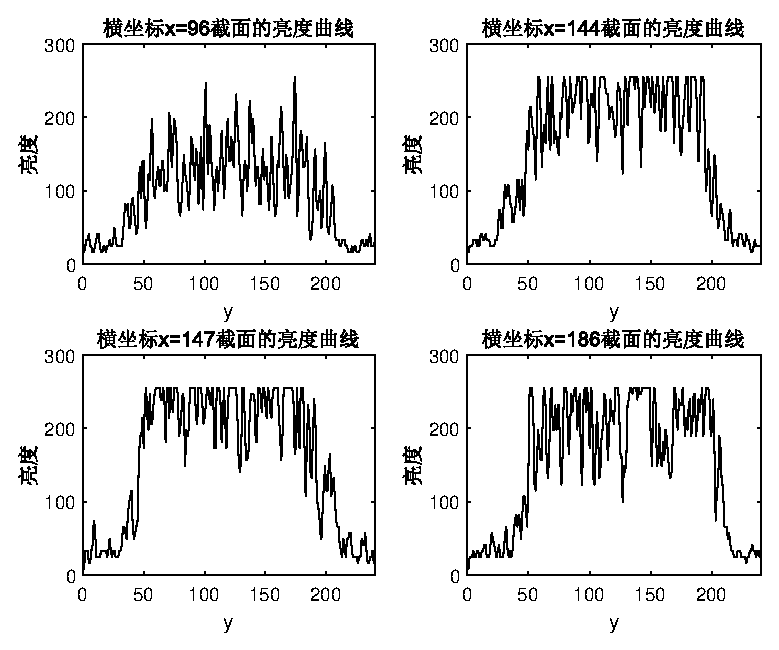
\includegraphics{addDOEmoveCCD25.eps}
		\caption{加DOE后平移在刻度25cm处亮度图}\label{fig-addDOEmoveCCD25}
	\end{figure}
	
	\section{思考题与讨论}
	\section{本实验的收获,体会和建议}
\end{document}
